\chapter{related Work / ähnliche Arbeiten}

Da Software-Testing ein stetig wachsendes Thema ist und der allgemeine Konsens \"man kann nicht genug testen\" existiert ist
es klar, dass diverse Arbeiten in Richtung Testautomatisierung erstellt wurden. In diesem Abschnitt sollen ähnliche Arbeiten
genannt werden sowie Unterschiede zu diesen Arbeiten benannt werden.

\section{EvoMaster}

EvoMaster ist ein Open-Source Tool welches sich automatisiertes Testen von Rest-APIs und GraphQL APIs zur Aufgabe gemacht hat.
Aktuell kann durch EvoMaster sowohl WhiteBox Testing als auch BlackBox Testing durchgeführt werden jedoch ist ein
Whitebox Test mittels Vanilla-EvoMaster nur für Rest-APIs möglich die mit der JVM lauffähig sind.
Im Paper \"White-Box and Black-Box Fuzzing for GraphQL APIs" (Quelle hier) wurde ein System on-Top für EvoMaster
erstellt welches GraphQL Tests generieren kann. Hierbei soll sowohl WhiteBox als auch BlackBox Testing möglich sein.
Das erstellte Framework in diesem Paper arbeitet nach folgendem Prinzip:

\begin{center}
    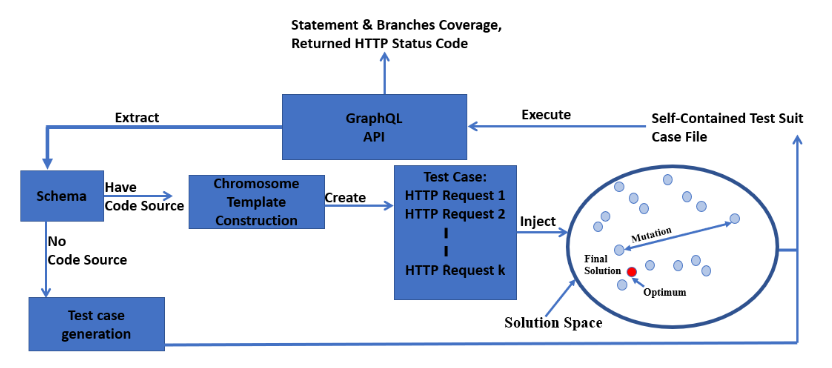
\includegraphics[width=\textwidth,height=\textheight,keepaspectratio]{content/hauptteil/related Work/evomaster_framework}
\end{center}

WhiteBox Testing ist möglich insofern Zugang zum GraphQL-Schema und zum Source Code der API gegeben ist. Andernfalls ist
nur BlackBox Testing möglich. Zur Testgenerierung wird ein genetischer Algorithmus genutzt welcher die Tests generiert.
Wie dieser genetische Algorithmus genau funktioniert kann im Paper selbst nachgelesen werden (hier Quelle).
Im Vergleich mit unserer geplanten Arbeit mittels des Prime-Path-Algorithmus ergeben sich einige Unterschiede, diese sind
unter anderem: Nutzung eines evolutionären Algorithmus Many-Independent-Objective (MIO).
Im Paper selbst wird davon ausgegangen, dass andere evolutionäre Algorithmen unter Umständen passender wären als der MIO Algorithmus
für die Testgenerierung. Jedoch ist ein evolutionärer Algorithmus auch immer ein stochastisch, heuristisch sich dem Optimum annähernder Algorithmus. (Beleg hierfür)
Im Gegensatz dazu ist der Ansatz dieser Arbeit ein natürlicher Algorithmus der beweisbar ideale Lösungen auf direkte Art bietet
und im ersten Durchlauf direkt sein ideales Ergebnis ermittelt. Die ideale Lösung bezieht sich hierbei auf bestimmte
Code-Coverage Kriterien die durch unseren Algorithmus erfüllt werden.  Inwiefern der evolutionäre Algorithmus diese
Kriterien erfüllt bleibt offen, es ist jedoch davon auszugehen, dass er sich einer idealen Lösung dieser Kriterien nur
annähert da er eben ein stochastischer Algorithmus ist. (beleg oder Quelle)

\section{Deviation Testing}

Da GraphQL dynamisch auf Anfragen reagiert und es somit möglich ist, in seiner Anfrage einzelne Felder mit einzubeziehen
oder auch auszuschließen ist dies im Grunde genommen ein einzelner Test-Case.
Im Paper \" Deviation Testing: A Test Case Generation Technique for GraphQL APIs" wird diese Gegebenheit benutzt und
aus einer selbstdefinierten Query werden hier einzelne Test-Cases gebildet. Ein solcher Test macht je nach Implementierung
der GraphQL-Resolver druchaus Sinn, da im Backend Felder durchaus zusammenhängen können und es Bugs geben kann wenn
Resolver fehlerhaft definiert sind. z.B. könnte folgende Definition zu solchen Fehlern führen:

(hier BSP mit Code einfügen)

Da Deviation Testing jedoch nur bestehende Tests erweitert um mögliche Felder mitzutesten werden hier keine neuen Tests generiert.
Durch Deviation Testing werden bestehende Tests nur erweitert allerdings muss eine Edge-Coverage gegeben sein damit diese Arbeit
ein zufriedenstellendes Ergebnis erzeugt. Eine Edge-Coverage in einem komplexen Graphen ist allerdings sehr wahrscheinlich
schwer umsetzbar mit manuellem Test schreiben. Eine Paarung von Edge-Coverage mit Deviation-Testing wäre sicherlich Interessant.
Genau so wäre es interessant Deviation Testing als Teil unserer Arbeit zu nutzen indem mit diesem Tool die Tests erweitert werden.
(initialer Plan war es, einfach immer alle Felder eines Nodes zu testen, hierdurch wäre es möglich auch alle Varianten noch zu testen)

\section{AutoGraphQL}

Klassisches Testen von Anwendungen beeinhaltet, dass möglichst das komplette System getestet wird bevor es verwendet wird.
Im Paper "Harvesting Production GraphQL Queries to Detect Schema Faults" wird ein gänzlich anderer Ansatz verfolgt.
Hierbei ist es nicht wichtig die gesamte GraphQL-API vor der Veröffentlichung zu testen sondern
echte Queries die in Production ausgeführt werden zu sammeln.
Der Ansatz der hierbei verfolgt wird begründet sich daraus,
dass ein Testraum für GraphQL potentiell unendlich sein kann und es sehr wahrscheinlich ist, dass nur ein kleiner
Teil der API wirklich intensiv genutzt wird, sodass auch nur dieser Teil wirklich stark durch Tests abgedeckt werden muss.
AutoGraphQL läuft hierbei in zwei Phasen wobei in der ersten Phase alle einzigartigen Anfragen geloggt werden.
In der zweiten Phase werden dann aus den geloggten Anfragen Tests generiert.
Hierbei wird für jede geloggte Query genau ein Test-Case erstellt.
Bei dieser Art des Testens wird insbesondere darauf Wert gelegt, dass es keine Fehler im GraphQL Schema gibt.
Dies ist ein wichtiger Teil um GraphQL-API's zu testen allerdings noch kein vollständiger Test denn hier wird außer Acht gelassen,
dass eine Query konform zum GraphQL-Schema sein kann aber trotzdem falsch indem zum Beispiel falsche Daten zurückgegeben werden
durch falsche Referenzierung oder ähnlichem.
In dem zu entwickelndem Tool sollten alle Querys die von AutoGraphQL geloggt werden auch berücksichtig werden da sie durch
den Prime-Path Algorithmus auch ermittelt werden.
Es kann allerdings sinnvoll sein AutoGraphQL als Monitoring-Software mitlaufen zu lassen und weitere etwaige Fehler hiermit zu loggen
und automatisch daraus Test-Cases erstellen zu können damit zukünftig keine Fehler dieser Art mehr passieren.


